\documentclass{article}

\usepackage{amsmath}

\usepackage{lmodern}

\usepackage{graphicx} 

\usepackage{fancyhdr}

\usepackage{subcaption}

\usepackage[margin=1.2in]{geometry} 

\setlength\headheight{10pt} 

\renewcommand{\figurename}{Figura}


\pagestyle{fancy}
\fancyhf{}
\cfoot{\thepage}
\rhead{Nicol�s Vald�s \\ RUT: 19.247.388-8 \\ FI3104-1 2018B \\ 4/10/18}
\lhead{
\includegraphics[scale=0.52]{logo}}



\begin{document}
\thispagestyle{fancy}
\text{} \vspace{0.3cm}
\begin{center}
\LARGE {\bf Tarea 2} 
\end{center}
\normalsize 
\section*{Problema 1}
\subsection*{Introducci�n} 

La catenaria %stuff about chains, etc

Su ecuaci�n est� dada por 
\begin{align}
y(x) = a\cosh\left(\frac{x-x_0}{a}\right),
\end{align}
donde
\subsection*{Metodolog�a} 

Escogemos $x_0=0$ por conveniencia. Por el enunciado sabemos que la diferencia de altura entre el punto medio y un extremo es $H = 7.5$ metros. La distancia horizontal entre estos dos puntos es $L = 10$ metros. Entonces tenemos la ecuaci�n 
\begin{align}
y(L)-y(0) = H \implies F(a) = 0,
\end{align}
donde 
\begin{align}
F(a)\equiv a\cosh\left(\frac{L}{a}\right) - a - H.
\end{align}
Entonces para encontrar $a$, debemos encontrar ra�ces de la funci�n $F$. 
\begin{figure}[ht!]
\centering
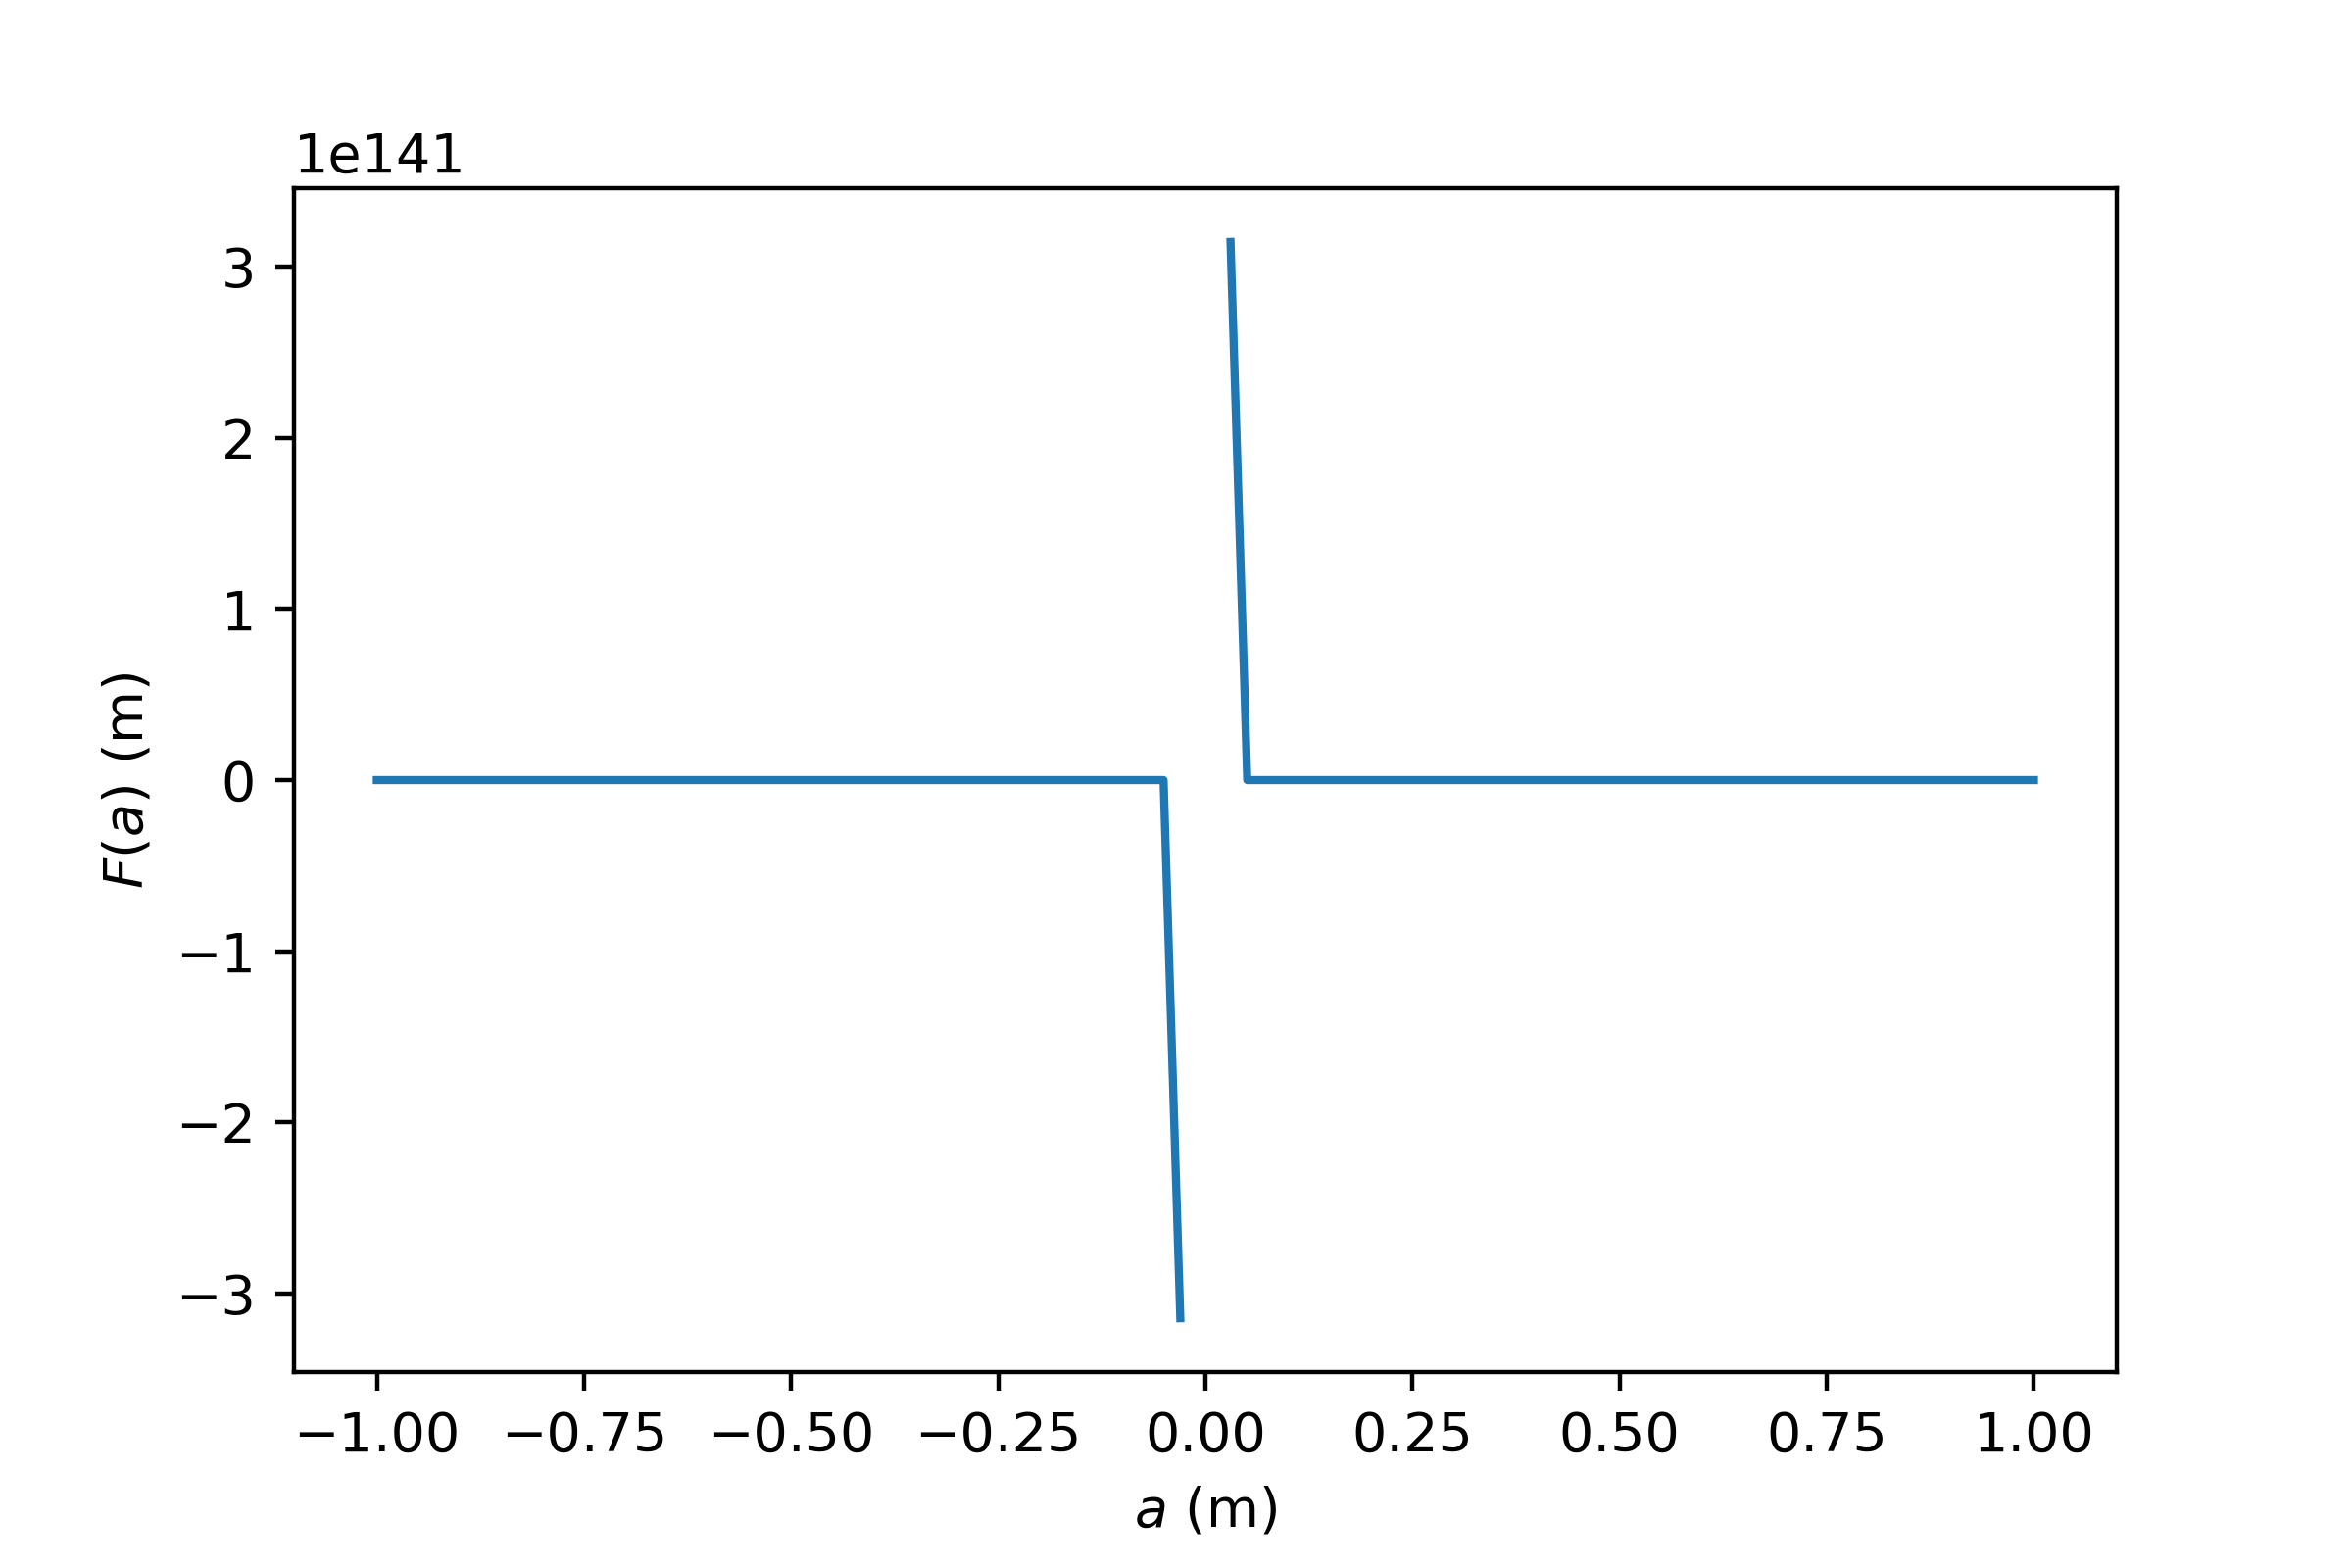
\includegraphics[width=3in]{ejemplo}
\caption{Gr�fico de $F(a)$}
\end{figure}

Viendo el gr�fico que hicimos de $F(a)$, est� claro que el m�todo de Newton no se debe usar. Se ve, primero, que diverge la funci�n en $a=0$, lo cu�l podr�a causar problemas. Adem�s, la derivada de la funci�n es un n�mero muy peque�o en la zona donde parece haber una ra�z de la funci�n. Dadas estas dos cosas, lo mejor parece ser utilizar el m�todo de la bisecci�n, comenzando con dos n�meros positivos para evitar una posible ra�z en el lado negativo, y para evitar la divergencia de $F$. 

\subsection*{Resultados} 



\subsection*{Conclusiones} 

%why newton's method
No usamos el m�todo de Newton para encontrar ra�ces de $F$ porque al tomar su derivada con respecto a $a$, notamos que $F'(a)=0$ cuando 
\begin{align}
\tanh\left(\frac{L}{a}\right) = \frac{a}{L}
\end{align}
Entonces a pesar de que la convergencia del m�todo de Newton es m�s r�pida que la del m�todo de bisecci�n, este segundo m�todo es m�s seguro en este caso. 
$F(a)$ no es una funci�n peri�dica, y es una funci�n cuya derivada siempre es positiva, salvo por los puntos $a=0$, $a=\infty$. Dado esto, el m�todo de Newton no deber�a tener problemas al funcionar. Adem�s, su convergencia es cuadr�tica a diferencia del m�todo de bisecci�n, por lo que es m�s eficiente. 

\section*{Problema 2}

\subsection*{Introducci�n} 



\subsection*{Metodolog�a} 


\subsection*{Resultados} 





\subsection*{Conclusiones} 



\section*{Mensaje Secreto} 
{\it
``In the beginning the Universe was created. This has made a lot of
people very angry and been widely regarded as a bad move.''}

\hfill-- Douglas Adams.\\
Esto lo encontr� en GitHub Desktop, meti�ndome a History y buscando en los distintos commits si hab�a un mensaje secreto. 





\end{document} 